\chapter{Experiments and Results} \label{chap:experiments}

\section{Gaussian Mixture Model Inverse Problem} \label{sec:gmm}

Beginning with an inverse problem, we consider the synthetic experiment described in
\textcite{cardosoMonteCarloGuided2023,boysTweedieMomentProjected2023}.
Consider a Gaussian mixture model (GMM), $p_{\text{data}}$, with 25 equally weighted
($\omega_{i,j} \propto 1$) $d_x$-dimensional Gaussian random variables with means
$\mathbf{\mu}_{i,j} := (8i, 8j, \dots, 8i, 8j) \in \mathbb{R}^{d_x}$
for $(i, j)\in \{-2, \ldots, 2\}^2$ and unit variance.
We generate some $d_y$-dimensional measurement, $\mathbf{y}$, according to the following process:
\begin{itemize}
    \item Draw $\tilde{A} \sim \mathcal{N}(0, 1)^{d_y \times d_x} \in \mathbb{R}^{d_y \times d_x}$
    and compute its SVD decomposition, $USV^\top$.
    \item Sample $s_{i,j} \sim \mathcal{U}[0,1]$ for $(i,j) \in \{-2, \dots, 2\}^2$.
    \item Set $A := U\, diag(\{s_{i,j}\})\, V^\top$.
    \item Draw $\mathbf{x}_* \sim p_{\text{data}}$ and set $\mathbf{y} := A\mathbf{x}_* + \sigma_y\epsilon,\ \epsilon \sim \mathcal{N}(\mathbf{0}_{d_y}, \mathrm{I}_{d_y})$
\end{itemize}

The goal of the inverse problem is to take $\mathbf{y}$ (with $A$ and $\sigma_y$ known), and use
it to infer $\mathbf{x}_*$. We consider $d_y < d_x$, making the problem ill-posed. Per
\autoref{rem:bayes-inv}, we tackle this by considering $p_{\text{data}}(\mathbf{x})$ as a prior
distribution,
$g(\mathbf{y} \mid \mathbf{x}) = \mathcal{N}(\mathbf{y}; A\mathbf{x}, \sigma_y\mathbf{I}_{d_y})$
as the measurement density, and then aim to sample from $p(\mathbf{x} \mid \mathbf{y})$.

For this model, given $p_{\text{data}}$ is available in closed form, the posterior,
$p(\mathbf{x}_* \mid \mathbf{y})$, is actually available in closed form as another GMM with:
\begin{align*}
    c_{i,j} &:= \mathcal{N}\left(\Sigma\left(\sigma_y^{-2}\cdot A^\top\mathbf{y} + \mu_{i,j}\right), \Sigma\right) \\
    \tilde{\omega}_{i,j} &\propto \omega_{i,j} \mathcal{N}\left(\mathbf{y}; A\mu_{i,j}, \mathbf{I}_{d_x} + AA^\top \right)
\end{align*}
with $\Sigma := \left(\mathbf{I}_{d_x} + \sigma_y^{-2}\cdot A^\top A\right)^{-1}$. This enables
us to accurately benchmark the different numerical methods.

Supposing $p_{\text{data}}$ was not available in closed form / easy to sample from, we may consider
using a diffusion model to sample from it. As $p_{\text{data}}$ is a GMM, the backwards marginal is
also available in closed form allowing us to avoid training a score network, being able to use
simple auto-differentiation of the marginal to yield the exact score at intermediate time-steps in a
diffusion process. Then using \autoref{eq:backwards-process}, we can sample from $p_{\text{data}}$
in some $T$ time-steps. In \autoref{fig:gmm-prior} we show prior samples from such an
unconditional model (compared with exact posterior samples for a particular inverse problem).

We can then apply our method, as described in \autoref{sec:inv-prob-spec-case}
with $\gamma(t) = 1$, to guide the process to enable sampling from the posterior,
$p(\mathbf{x} \mid \mathbf{y})$. We can contrast \texttt{SMCDiffOpt} numerically with the
non-particle based approaches of
\textcite{song2023pseudoinverseguided,boysTweedieMomentProjected2023,chungDiffusionPosteriorSampling2022}
\footnote{See \autoref{sec:experimental-extra} for discussion as why MCGdiff comparison was excluded.},
using sliced-Wasserstein distance \parencite{boysTweedieMomentProjected2023,cardosoMonteCarloGuided2023}
to measure how well each method approximates the true posterior distribution based on samples
drawn directly from it.

\begin{table}[t]
    \centering
    \begin{tabular}{llllll}
        \toprule
        $d_x$ & $d_y$ & SMCDiffOpt & DPS & $\Pi$IGD & TMPD \\
        \midrule
        \multirow[t]{3}{*}{8} & 1 & 1.35 ± 1.0 & 8.18 ± 7.5 & 3.16 ± 2.72 & 3.31 ± 2.86 \\
         & 2 & 0.55 ± 0.43 & 2.72 ± 2.62 & 0.94 ± 0.89 & 1.34 ± 1.25 \\
         & 4 & 0.19 ± 0.09 & 0.95 ± 0.9 & 0.09 ± 0.03 & 0.37 ± 0.33 \\
        \cline{1-6}
        \multirow[t]{3}{*}{80} & 1 & 1.65 ± 1.41 & 5.03 ± 4.63 & 3.08 ± 2.71 & 2.42 ± 1.71 \\
         & 2 & 1.19 ± 1.07 & 3.14 ± 3.02 & 1.68 ± 1.62 & 1.35 ± 1.22 \\
         & 4 & 1.11 ± 0.93 & 1.32 ± 1.21 & 0.84 ± 0.79 & 1.14 ± 0.9 \\
        \cline{1-6}
        \bottomrule
    \end{tabular}
    \caption{Sliced-Wasserstein distances of samples from particle samples.}
    \label{tab:gmm}
\end{table}

We experiment for $d_x \in \{8, 80\}$, $d_y \in \{1, 2, 4\}$, and $\sigma_y \in \{0.01, 0.1, 1.0\}$,
comparing the performance of \texttt{SMCDiffOpt}, diffusion-posterior-sampling (DPS;
\cite{chungDiffusionPosteriorSampling2022}), pseudo-inverse-guided-diffusion ($\Pi$IGD;
\cite{song2023pseudoinverseguided}), and Tweedie-moment-projected-diffusion (TMPD;
\cite{boysTweedieMomentProjected2023}). We run the experiment for 10 different seeds,
generating 10 different measurement models according to the above steps, using 1000
particles for \texttt{SMCDiffOpt} and generating 1000 independent samples for the other methods,
all in 1000 time-steps under DDPM sampling.

\begin{figure}[t]
    \centering
    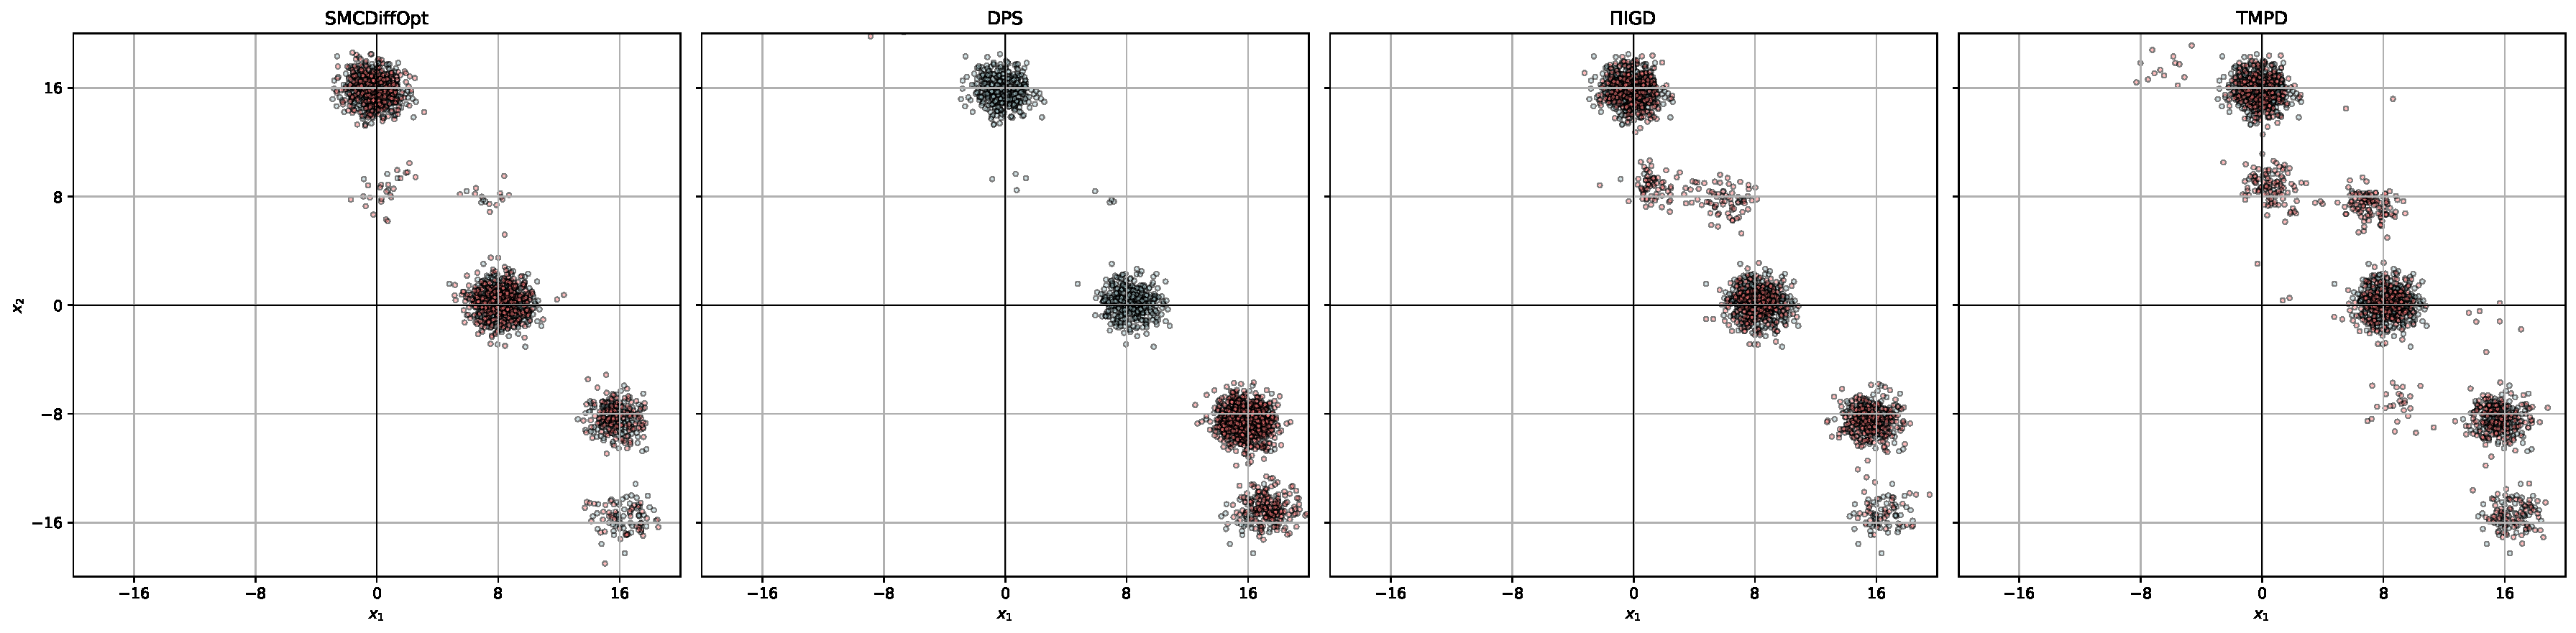
\includegraphics[width=1\textwidth]{assets/gmm_samples.pdf}
    \caption{Comparison of samples against true posterior samples; $d_x = 8; d_y = 2$.}
    \label{fig:gmm-samples}
\end{figure}

The results are shown in \autoref{tab:gmm} rolled up on $\sigma_y$; in \autoref{tab:gmm-sigma-split} we
show the full-results split out by $\sigma_y$\footnote{This table roughly aligns with Table 4 of
\textcite{boysTweedieMomentProjected2023}, providing some level of validation.}. The values shown
are the median and ranges for the sliced-Wasserstein distance over the seeds. We see
that \texttt{SMCDiffOpt} outperforms the other methods. In \autoref{fig:gmm-samples} we plot the
first two co-ordinates of the samples generated by each method overlaying true posterior samples for
a specific measurement model with $d_x = 8, d_y = 2$, providing visual confirmation.
\autoref{fig:gmm-prior-smc-samples} better highlights how \texttt{SMCDiffOpt} is able to accurately
guide the unconditional sampler to instead sample from the posterior.

\begin{figure}[t]
    \centering
    \begin{subfigure}[b]{0.48\textwidth}
      \centering
      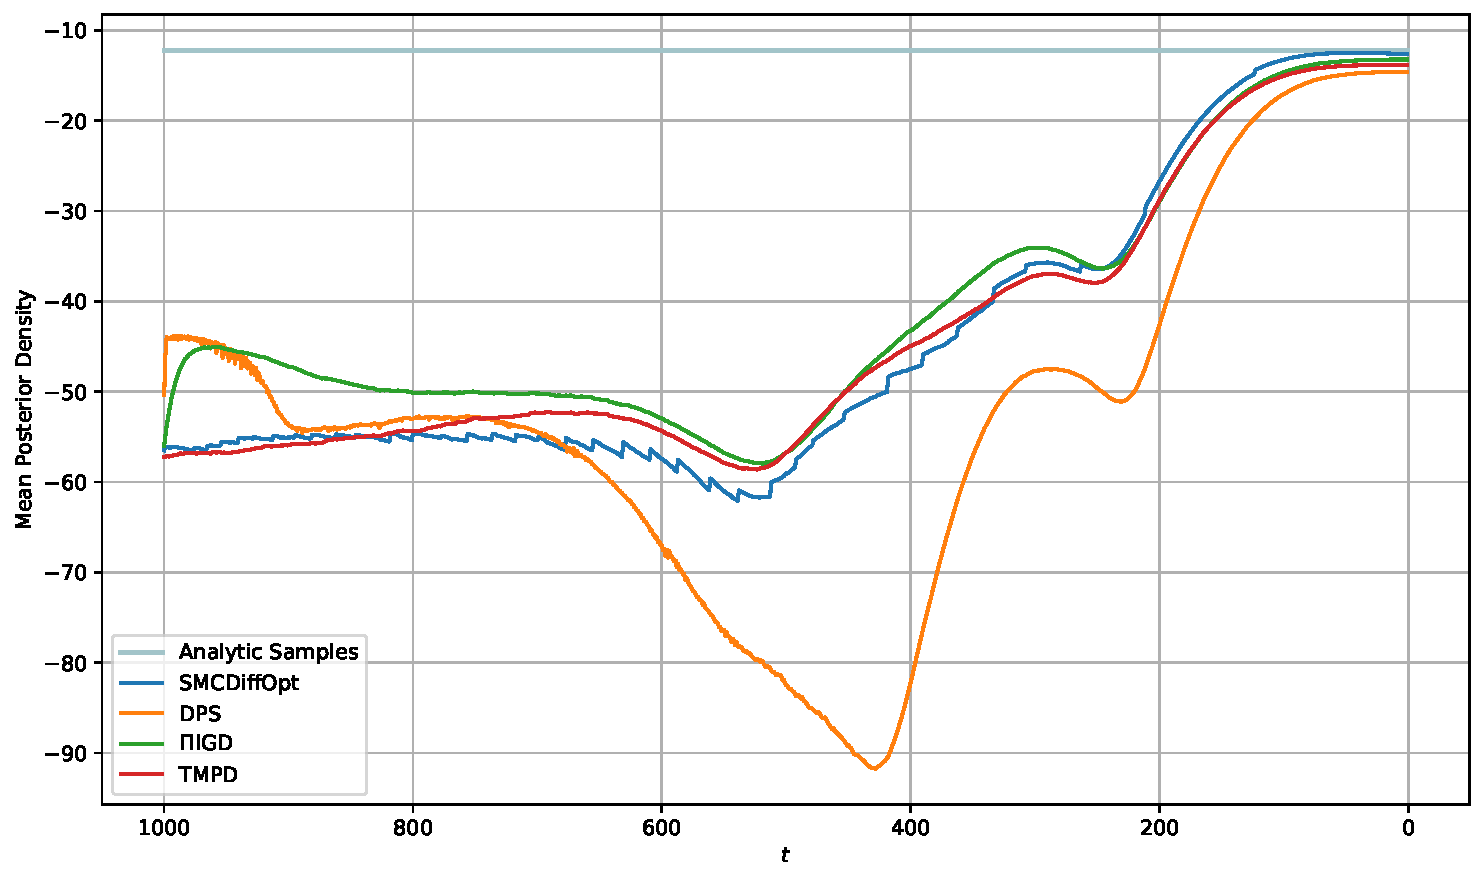
\includegraphics[width=\textwidth]{assets/gmm_posterior_densities.pdf}
      \caption{Log-Posterior density over time.}
      \label{fig:gmm-posterior}
    \end{subfigure}
    \hfill
    \begin{subfigure}[b]{0.48\textwidth}
      \centering
      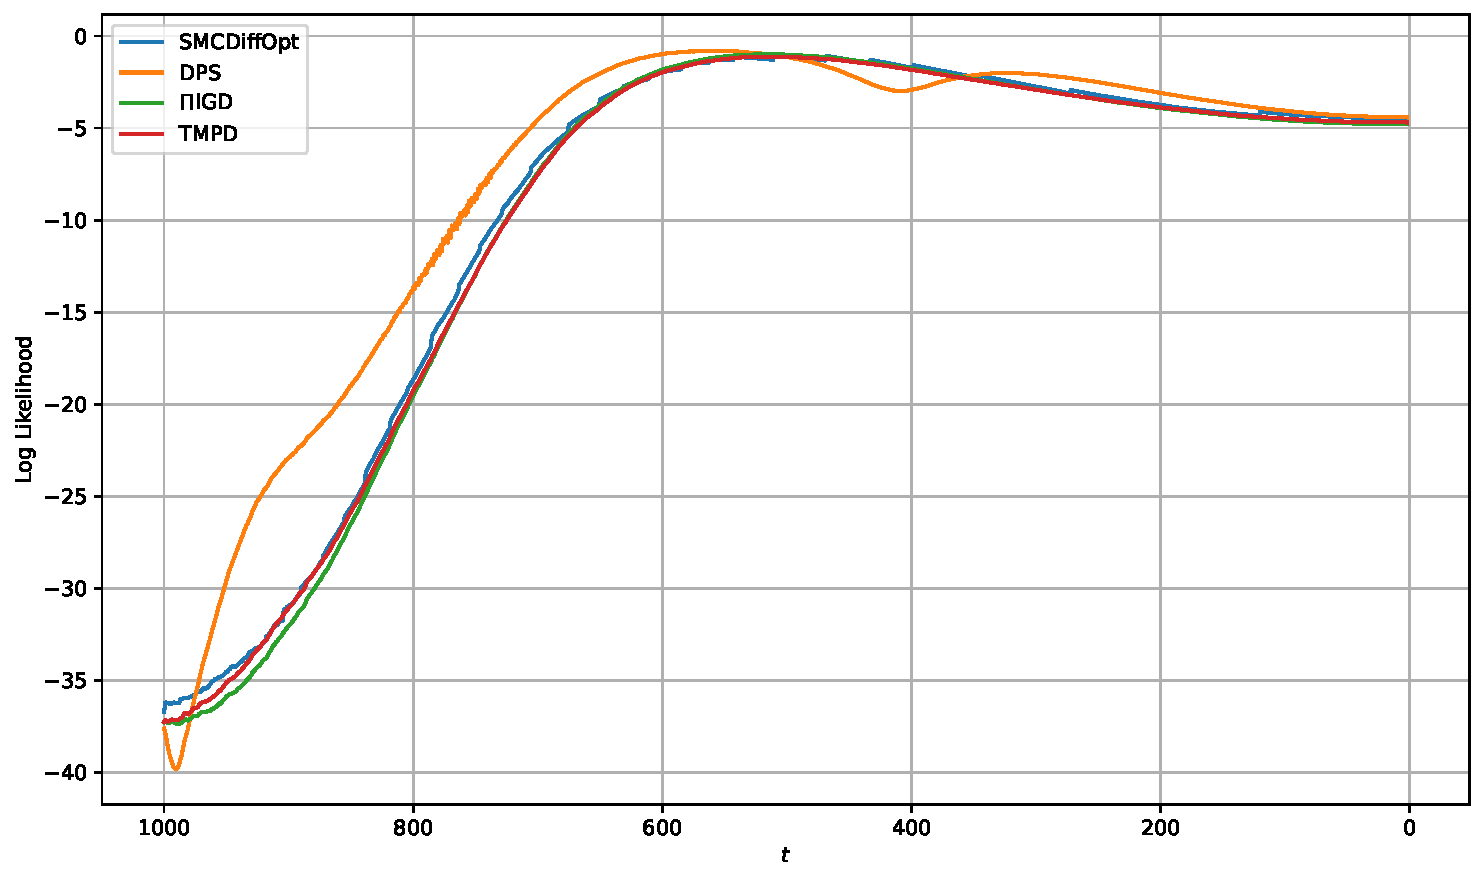
\includegraphics[width=\textwidth]{assets/gmm_log_likelihoods.pdf}
      \caption{Log-Likelihood over time.}
      \label{fig:gmm-log-likelihoods}
    \end{subfigure}
    \caption{Mean log-posterior and log-likelihood of samples over time with respect to
    observations, $\{\mathbf{y}_t\}_{t=1}^T$, constructed per \autoref{eq:obs-gen}; associated with
    \autoref{fig:gmm-samples}.}
    \label{fig:gmm-metrics}
\end{figure}

In \autoref{fig:gmm-metrics} we show the evolution of the true (log) posterior density evaluated on the
sample at step $t$, $p_{\mathbf{x}_0 \mid \mathbf{y}}(\mathbf{x}_t \mid \mathbf{y})$, and (log)
likelihood, $g(\mathbf{y}_t \mid \mathbf{x}_t)$, over the course of the guided diffusions under
each method. \autoref{fig:gmm-posterior} shows how well the methods ultimately target the posterior
distribution; we see that all but DPS follow similar trajectories.
Examining \autoref{fig:gmm-log-likelihoods} in conjunction, we see that the methods appear to operate
by first optimizing the likelihood to a point before turning to optimize the posterior density,
allowing the likelihood to decline. Essentially, \autoref{fig:gmm-metrics} highlights the regularization
effect of the diffusion prior model.

Note that the numeric comparison of \texttt{SMCDiffOpt} with the other three methods isn't entirely
fair since the former is an interacting-particle algorithm; \texttt{SMCDiffOpt} requires several
particles to operates whereas the others are independent runs. Reducing the number of particles
will almost definitionally reduce the relative outperformance of \texttt{SMCDiffOpt} over the
others. This provides an interesting avenue for future research in the form of an ablation study.

\section{Branin Function Optimization} \label{sec:branin}

\begin{figure}[t]
    \centering
    \begin{subfigure}[b]{0.48\textwidth}
        \centering
        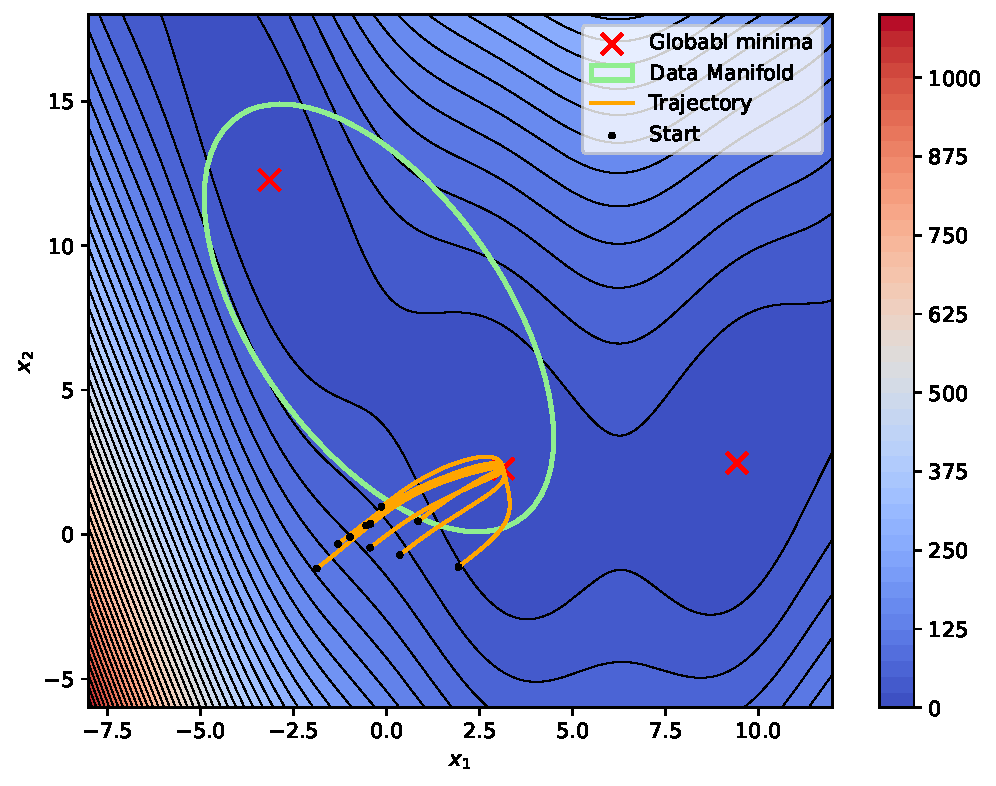
\includegraphics[width=1\textwidth]{assets/adam_branin.pdf}
        \caption{Adam with $\mathcal{N}(0, \mathbf{I}_{d_x})$ initialisation.}
        \label{fig:branin-adam-a}
    \end{subfigure}
    \hfill
    \begin{subfigure}[b]{0.48\textwidth}
        \centering
        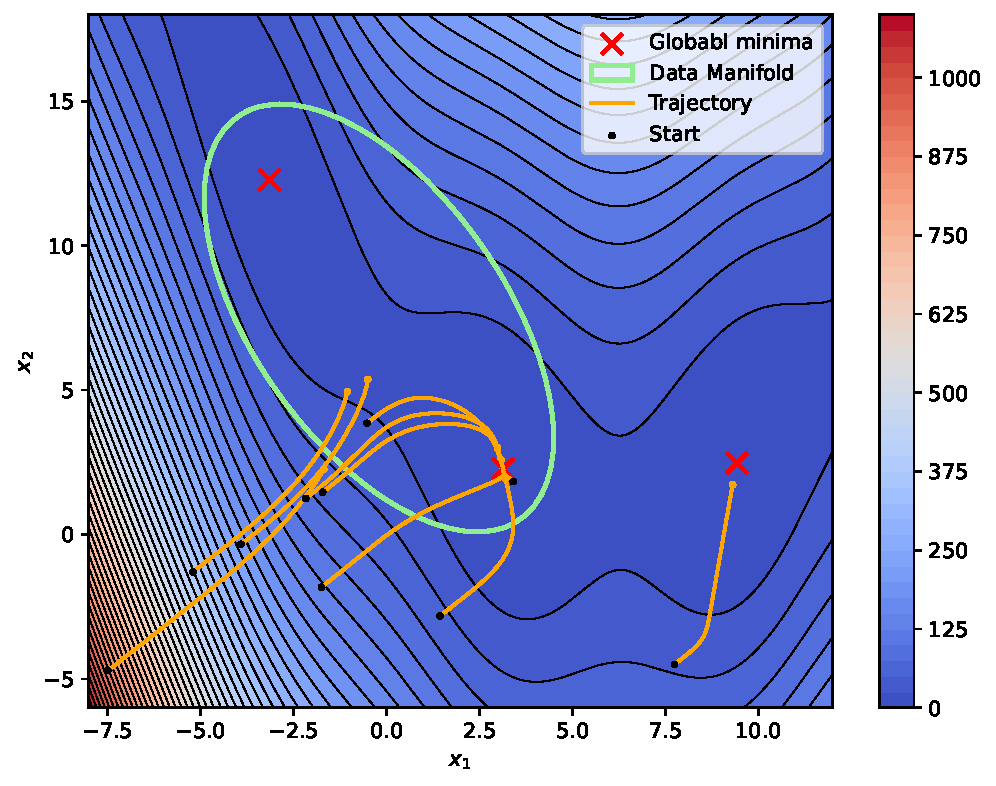
\includegraphics[width=1\textwidth]{assets/adam_larger_branin.pdf}
        \caption{Adam with $\mathcal{N}(0, 16\cdot\mathbf{I}_{d_x})$ initialisation.}
        \label{fig:branin-adam-b}
    \end{subfigure}
    \caption{Pitfalls of naieve gradient optimisation of the Branin function.}
    \label{fig:branin-adam}
\end{figure}

For a general optimization task, we consider optimizing the Branin function as an objective over
some constrained region (the data manifold) as detailed in
\textcite{kongDiffusionModelsConstrained2024}. The Branin function is defined by:
\begin{equation}
    f(x_1, x_2) = a(x_2 - bx_1^2 + cx_1 - r)^2 + s(1-t)\cos(x_1) + s \label{eq:branin}
\end{equation}
where $a=1$, $b = \frac{5.1}{4\pi^2}$, $c=\frac{5}{\pi}$, $r=6$, $s=10$, $t=\frac{1}{8\pi}$.
It has three global minima located at $(-\pi, 12.275)$, $(\pi, 2.275)$ and $(9.42478, 2.475)$,
with a value of $0.397887$. We consider some uniform prior sampling distribution, $p_{\text{data}}$,
over an ellipse region centred at $(-0.2, 7.5)$ with semi-axis lengths $(3.6, 8)$, tilted
$25^\circ$. This region covers two of the global minima $(-\pi, 12.275)$ and $(\pi, 2.275)$.
See \autoref{fig:branin-adam} to visualize.

Similar to in \autoref{sec:gmm}, here we can easily sample from $p_{\text{data}}$ by inverse-transform
sampling. Again, we suppose now that we can't do so and suppose also that we're in a high-dimensional
setting where performing a simple visual analysis to quickly infer the geometry of the objective
function and data manifold is not possible. Our stated objective is to optimize the function over
the data manifold, ideally finding the $(-\pi, 12.275)$ and $(\pi, 2.275)$ points, but \emph{not}
the $(9.42478, 2.475)$ point (since it's outside the constrained region / not a \emph{valid
configuration}).

The obvious approach might be to use a gradient-based optimizer, such as the popular
Adam \parencite{kingmaAdamMethodStochastic2017}, adaptive-moment-estimating optimizer. However,
without prior knowledge of the data manifold, choosing initial points for the optimizer is
challenging. In \autoref{fig:branin-adam-a} we show choosing 10 (for visual clarity) starting points
randomly from a $\mathcal{N}(0, \mathbf{I}_{d_x})$ distribution. Using a base learning rate of
$0.05$ and 1000 iterations of the optimizer, we see that in this case the optimizer does find one of
the optima, but has essentially no chance of finding the other. In \autoref{fig:branin-adam-b} we re-run
the optimizer but with initial points randomly from a $\mathcal{N}(0, 16\cdot\mathbf{I}_{d_x})$
distribution instead. Here we see that while the optimizer found the two desired points, it also found
one of the points outside the constrained region --- an invalid configuration. Furthermore, we see
that one of trajectories didn't converge to an optima; this sample headed towards the saddle-point
region between the two optima and essentially got stuck there requiring many iterations to escape.
The key issue here is that the optimizer has no guidance towards the data manifold and relies solely
on the gradient. Obviously, if we could sample from $p_{\text{data}}$ analytically, choosing this as
the distribution to pick initial samples is optimal. Since we can't generally, we resort to
generative techniques, such as diffusion models.

\begin{figure}[t]
    \centering
    \begin{subfigure}[b]{0.48\textwidth}
        \centering
        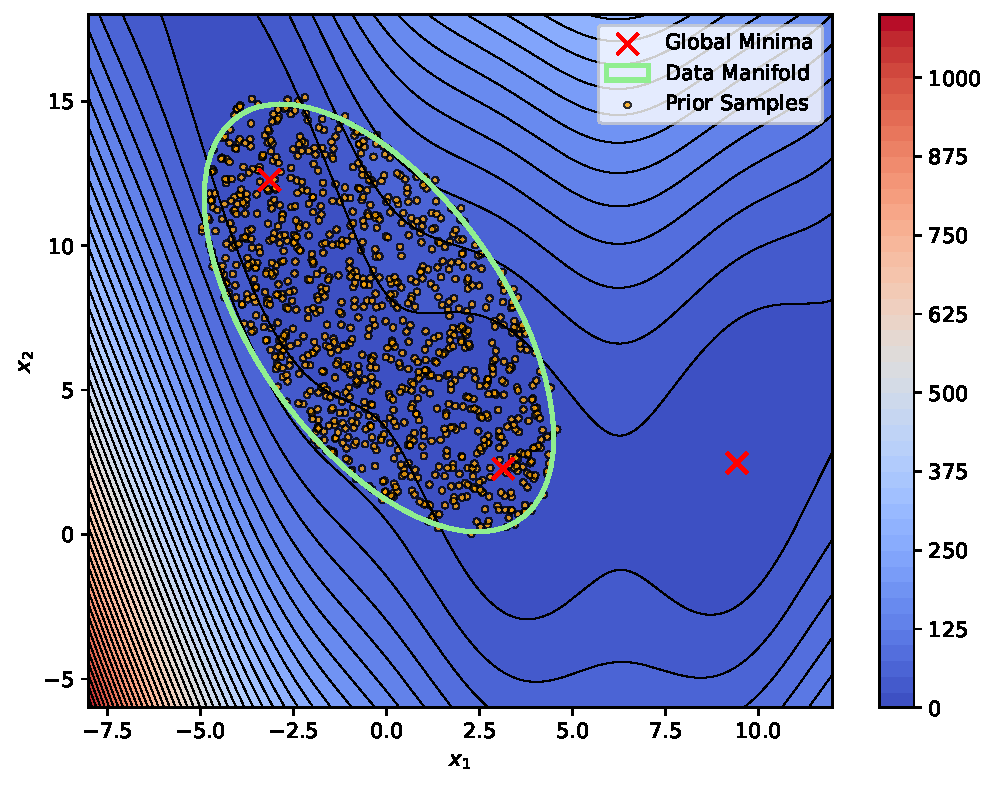
\includegraphics[width=1\textwidth]{assets/smc_branin_prior.pdf}
        \caption{Prior samples from trained model well-targetting the data manifold.}
        \label{fig:branin-prior}
    \end{subfigure}
    \hfill
    \begin{subfigure}[b]{0.48\textwidth}
        \centering
        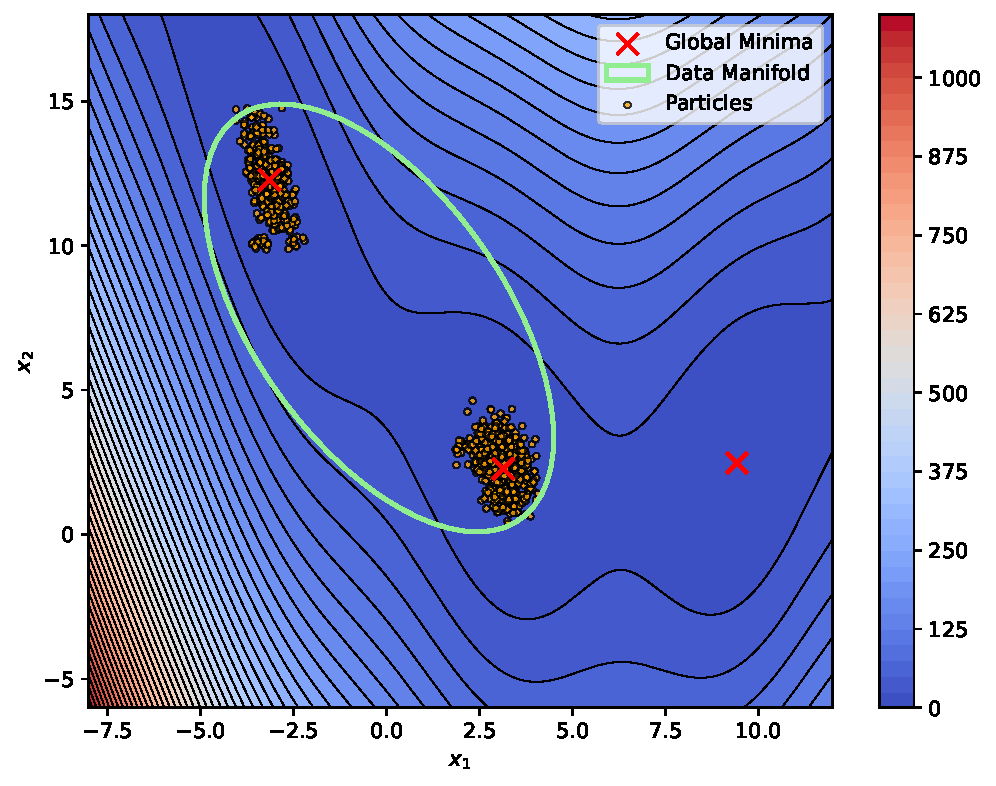
\includegraphics[width=1\textwidth]{assets/smc_branin.pdf}
        \caption{\texttt{SMCDiffOpt}'s resulting particles from optimizing the Branin function.}
        \label{fig:branin-smc}
    \end{subfigure}
    \caption{Prior versus optimised samples under guidance through \texttt{SMCDiffOpt}.}
    \label{fig:branin-prior-smc}
\end{figure}

To apply \texttt{SMCDiffOpt}, we sample training data from $p_{\text{data}}$\footnote{Obviously, we
are supposing this sampling isn't generally possible; we are in a generative modelling situation
where we pre-suppose access to a finite number of samples from $p_{\text{data}}$ a priori, and
train a model on these, hoping it enables general sampling from $p_{\text{data}}$.}, and use this
to train a simple score-based diffusion model (details in \autoref{sec:experimental-extra}). With such
a model, we can now approximately generate samples from $p_{\text{data}}$. More importantly, we can
use the model as a prior, using it as transition kernel in \autoref{alg:smc-opt}, with the `likelihood'
being an (annealed) induced Boltzmann distribution from the Branin function. Choosing
$\gamma(t) = 1 - e^{-\zeta T}$ for some small, tunable $\zeta$ (e.g. $0.001$), we run
\autoref{alg:smc-opt} with 1000 particles. In \autoref{fig:branin-smc}, we see that the procedure has
well-discovered the two desired optima; using the final particle weights the precise global minima
can be easily discovered. This is further highlighted in \autoref{fig:branin-mean-val} where we show
how the mean Branin value across the particles evolves over time.

The remarkable feature of \autoref{alg:smc-opt} is that it can achieve this optimisation without
requiring access to the gradient of the objective. As mentioned in \autoref{chap:methods}, if we did
have access to these gradients we could consider using them with \autoref{alg:smc-opt} either as an
additional step after moving the particles
(``gradient nudging'' \parencite{akyildizNudgingParticleFilter2020}) or as a means of picking a
better proposal distribution (``twisting'' \parencite{wuPracticalAsymptoticallyExact2023}). In
such cases, the requisite number of particles and the reliance on the $\gamma(t)$ schedule should
likely reduce.

\section{Black-Box Optimization} \label{sec:superconductor}

For a black-box optimisation task, we consider the SuperConductor task of
\textcite{trabuccoDesignBenchBenchmarksDataDriven2022}. Originally proposed in
\textcite{HAMIDIEH2018346}, the goal is ``to design a chemical formula for a superconducting
material that has a high critical temperature'' \parencite{trabuccoDesignBenchBenchmarksDataDriven2022}.
The dataset comprises 21,263 86-dimensional vectors and their associated critical temperatures. Each
component of the vector represents the ``mixture of elements by number of atoms in the chemical
formula of each superconductor'' \parencite{trabuccoDesignBenchBenchmarksDataDriven2022}. A provided
oracle model takes any configuration and gives the associated temperature. This is the black-box
function we wish to optimize; we want to find the vector which maximizes the oracle.

As suggested in \textcite{trabuccoDesignBenchBenchmarksDataDriven2022}, and applied in
\textcite{kongDiffusionModelsConstrained2024,krishnamoorthyDiffusionModelsBlackBox2023},
we use an 80\% subset of the data for training. This holds out rows with the top and bottom 10\% of
temperatures. Training a score network on this data, the hope is this well models the data manifold
(allowed configurations) enabling it to act as a strong prior model for optimization. In
\autoref{fig:bb-samples} we show an example of a true sample (\autoref{fig:bb-real}) versus a sample
generated by the model (\autoref{fig:bb-unconditional}). Details of the model's architecture are
described in \autoref{sec:experimental-extra}.

Using this model, we can employ \texttt{SMCDiffOpt} for finding an optimal configuration. We can
determine the performance of \texttt{SMCDiffOpt} by yielding an optimised temperature from its final
particles (e.g. via sampling and evaluation, or evaluation then averaging; we choose latter for
benchmark comparisons). We min-max normalize such a score based on the full dataset to give a more
interpretable score; the maximum temperature in the whole dataset is 185 and the minimum is
$\approx 0$. We run the algorithm with annealing as in \autoref{sec:branin}, using only 100 particles.

As in \textcite{krishnamoorthyDiffusionModelsBlackBox2023}, we benchmark our approach with multiple
baselines including ``canonical approaches'' like gradient ascent and REINFORCE
\parencite{NIPS1999_464d828b}, the CMA-ES \parencite{Hansen2006} evolutionary strategy, and the CbAS
\parencite{pmlr-v97-brookes19a} and MINs \parencite{NEURIPS2020_373e4c5d} recent deep learning
methods. We also include the diffusion-based DDOM
\parencite{krishnamoorthyDiffusionModelsBlackBox2023} and DiffOpt
\parencite{kongDiffusionModelsConstrained2024} methods in our comparison. In
\autoref{tab:superconductor-norm} we present for each method the mean min-max normalised scores and
their 95\% CLT confidence intervals based on 5 runs of each on different random seeds. We see that
\texttt{SMCDiffOpt} comfortably outperforms each method, yielding state-of-the-art performance. We
show an example configuration generated by the optimizer in \autoref{fig:bb-optimised}.

\begin{table}[t]
    \centering
    \resizebox{\textwidth}{!}{
    \begin{tabular}{llllllll}
        \toprule
        CbAS & CMA-ES & Gradient Ascent & MINs & REINFORCE & DDOM & DiffOpt & \textbf{SMCDiffOpt} \\
        \midrule
        0.433 ± 0.027 & 0.474 ± 0.021 & 0.510 ± 0.009 & 0.473 ± 0.003 & 0.483 ± 0.015 & 0.560 ± 0.044 & 0.614 ± 0.029 & \textbf{0.644 ± 0.024} \\
        \bottomrule
    \end{tabular}
    }
    \caption{Normalized scores for SuperConductor experiment.}
    \label{tab:superconductor-norm}
\end{table}

Like in \autoref{sec:gmm}, the comparison is not exactly fair since our method uses 100
interacting particles compared to the other methods which are independent `samplers'. In black-box
settings, this can be a major downside since we may have a strict `query budget'
\parencite{krishnamoorthyDiffusionModelsBlackBox2023}, only being allowed to evaluate the oracle
a finite number of times. In such settings, \texttt{SMCDiffOpt} is generally ill-suited;
\hyperref[rem:time-respacing]{time-respacing}, gradient-nudging, or supplementary Langevin steps may
provide remedies but we defer investigating applying these ideas to future research.
